\documentclass[1p]{elsarticle_modified}
%\bibliographystyle{elsarticle-num}

%\usepackage[colorlinks]{hyperref}
%\usepackage{abbrmath_seonhwa} %\Abb, \Ascr, \Acal ,\Abf, \Afrak
\usepackage{amsfonts}
\usepackage{amssymb}
\usepackage{amsmath}
\usepackage{amsthm}
\usepackage{scalefnt}
\usepackage{amsbsy}
\usepackage{kotex}
\usepackage{caption}
\usepackage{subfig}
\usepackage{color}
\usepackage{graphicx}
\usepackage{xcolor} %% white, black, red, green, blue, cyan, magenta, yellow
\usepackage{float}
\usepackage{setspace}
\usepackage{hyperref}

\usepackage{tikz}
\usetikzlibrary{arrows}

\usepackage{multirow}
\usepackage{array} % fixed length table
\usepackage{hhline}

%%%%%%%%%%%%%%%%%%%%%
\makeatletter
\renewcommand*\env@matrix[1][\arraystretch]{%
	\edef\arraystretch{#1}%
	\hskip -\arraycolsep
	\let\@ifnextchar\new@ifnextchar
	\array{*\c@MaxMatrixCols c}}
\makeatother %https://tex.stackexchange.com/questions/14071/how-can-i-increase-the-line-spacing-in-a-matrix
%%%%%%%%%%%%%%%

\usepackage[normalem]{ulem}

\newcommand{\msout}[1]{\ifmmode\text{\sout{\ensuremath{#1}}}\else\sout{#1}\fi}
%SOURCE: \msout is \stkout macro in https://tex.stackexchange.com/questions/20609/strikeout-in-math-mode

\newcommand{\cancel}[1]{
	\ifmmode
	{\color{red}\msout{#1}}
	\else
	{\color{red}\sout{#1}}
	\fi
}

\newcommand{\add}[1]{
	{\color{blue}\uwave{#1}}
}

\newcommand{\replace}[2]{
	\ifmmode
	{\color{red}\msout{#1}}{\color{blue}\uwave{#2}}
	\else
	{\color{red}\sout{#1}}{\color{blue}\uwave{#2}}
	\fi
}

\newcommand{\Sol}{\mathcal{S}} %segment
\newcommand{\D}{D} %diagram
\newcommand{\A}{\mathcal{A}} %arc


%%%%%%%%%%%%%%%%%%%%%%%%%%%%%5 test

\def\sl{\operatorname{\textup{SL}}(2,\Cbb)}
\def\psl{\operatorname{\textup{PSL}}(2,\Cbb)}
\def\quan{\mkern 1mu \triangleright \mkern 1mu}

\theoremstyle{definition}
\newtheorem{thm}{Theorem}[section]
\newtheorem{prop}[thm]{Proposition}
\newtheorem{lem}[thm]{Lemma}
\newtheorem{ques}[thm]{Question}
\newtheorem{cor}[thm]{Corollary}
\newtheorem{defn}[thm]{Definition}
\newtheorem{exam}[thm]{Example}
\newtheorem{rmk}[thm]{Remark}
\newtheorem{alg}[thm]{Algorithm}

\newcommand{\I}{\sqrt{-1}}
\begin{document}

%\begin{frontmatter}
%
%\title{Boundary parabolic representations of knots up to 8 crossings}
%
%%% Group authors per affiliation:
%\author{Yunhi Cho} 
%\address{Department of Mathematics, University of Seoul, Seoul, Korea}
%\ead{yhcho@uos.ac.kr}
%
%
%\author{Seonhwa Kim} %\fnref{s_kim}}
%\address{Center for Geometry and Physics, Institute for Basic Science, Pohang, 37673, Korea}
%\ead{ryeona17@ibs.re.kr}
%
%\author{Hyuk Kim}
%\address{Department of Mathematical Sciences, Seoul National University, Seoul 08826, Korea}
%\ead{hyukkim@snu.ac.kr}
%
%\author{Seokbeom Yoon}
%\address{Department of Mathematical Sciences, Seoul National University, Seoul, 08826,  Korea}
%\ead{sbyoon15@snu.ac.kr}
%
%\begin{abstract}
%We find all boundary parabolic representation of knots up to 8 crossings.
%
%\end{abstract}
%\begin{keyword}
%    \MSC[2010] 57M25 
%\end{keyword}
%
%\end{frontmatter}

%\linenumbers
%\tableofcontents
%
\newcommand\colored[1]{\textcolor{white}{\rule[-0.35ex]{0.8em}{1.4ex}}\kern-0.8em\color{red} #1}%
%\newcommand\colored[1]{\textcolor{white}{ #1}\kern-2.17ex	\textcolor{white}{ #1}\kern-1.81ex	\textcolor{white}{ #1}\kern-2.15ex\color{red}#1	}

{\Large $\underline{12n_{0400}~(K12n_{0400})}$}

\setlength{\tabcolsep}{10pt}
\renewcommand{\arraystretch}{1.6}
\vspace{1cm}\begin{tabular}{m{100pt}>{\centering\arraybackslash}m{274pt}}
\multirow{5}{120pt}{
	\centering
	\includegraphics[width=112pt]{../../../GIT/diagram.site/Diagrams/png/2489_12n_0400.png}\\
\ \ \ A knot diagram\footnotemark}&
\allowdisplaybreaks
\textbf{Linearized knot diagam} \\
\cline{2-2}
 &
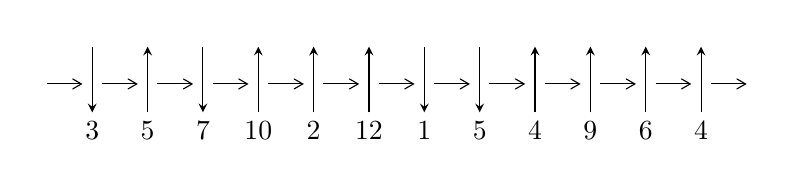
\begin{tikzpicture}[x=20pt, y=17pt]
	% nodes
	\node (C0) at (0, 0) {};
	\node (C1) at (1, 0) {};
	\node (C1U) at (1, +1) {};
	\node (C1D) at (1, -1) {3};

	\node (C2) at (2, 0) {};
	\node (C2U) at (2, +1) {};
	\node (C2D) at (2, -1) {5};

	\node (C3) at (3, 0) {};
	\node (C3U) at (3, +1) {};
	\node (C3D) at (3, -1) {7};

	\node (C4) at (4, 0) {};
	\node (C4U) at (4, +1) {};
	\node (C4D) at (4, -1) {10};

	\node (C5) at (5, 0) {};
	\node (C5U) at (5, +1) {};
	\node (C5D) at (5, -1) {2};

	\node (C6) at (6, 0) {};
	\node (C6U) at (6, +1) {};
	\node (C6D) at (6, -1) {12};

	\node (C7) at (7, 0) {};
	\node (C7U) at (7, +1) {};
	\node (C7D) at (7, -1) {1};

	\node (C8) at (8, 0) {};
	\node (C8U) at (8, +1) {};
	\node (C8D) at (8, -1) {5};

	\node (C9) at (9, 0) {};
	\node (C9U) at (9, +1) {};
	\node (C9D) at (9, -1) {4};

	\node (C10) at (10, 0) {};
	\node (C10U) at (10, +1) {};
	\node (C10D) at (10, -1) {9};

	\node (C11) at (11, 0) {};
	\node (C11U) at (11, +1) {};
	\node (C11D) at (11, -1) {6};

	\node (C12) at (12, 0) {};
	\node (C12U) at (12, +1) {};
	\node (C12D) at (12, -1) {4};
	\node (C13) at (13, 0) {};

	% arrows
	\draw[->,>={angle 60}]
	(C0) edge (C1) (C1) edge (C2) (C2) edge (C3) (C3) edge (C4) (C4) edge (C5) (C5) edge (C6) (C6) edge (C7) (C7) edge (C8) (C8) edge (C9) (C9) edge (C10) (C10) edge (C11) (C11) edge (C12) (C12) edge (C13) ;	\draw[->,>=stealth]
	(C1U) edge (C1D) (C2D) edge (C2U) (C3U) edge (C3D) (C4D) edge (C4U) (C5D) edge (C5U) (C6D) edge (C6U) (C7U) edge (C7D) (C8U) edge (C8D) (C9D) edge (C9U) (C10D) edge (C10U) (C11D) edge (C11U) (C12D) edge (C12U) ;
	\end{tikzpicture} \\
\hhline{~~} \\& 
\textbf{Solving Sequence} \\ \cline{2-2} 
 &
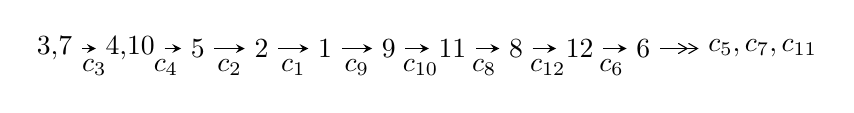
\begin{tikzpicture}[x=23pt, y=7pt]
	% node
	\node (A0) at (-1/8, 0) {3,7};
	\node (A1) at (17/16, 0) {4,10};
	\node (A2) at (17/8, 0) {5};
	\node (A3) at (25/8, 0) {2};
	\node (A4) at (33/8, 0) {1};
	\node (A5) at (41/8, 0) {9};
	\node (A6) at (49/8, 0) {11};
	\node (A7) at (57/8, 0) {8};
	\node (A8) at (65/8, 0) {12};
	\node (A9) at (73/8, 0) {6};
	\node (C1) at (1/2, -1) {$c_{3}$};
	\node (C2) at (13/8, -1) {$c_{4}$};
	\node (C3) at (21/8, -1) {$c_{2}$};
	\node (C4) at (29/8, -1) {$c_{1}$};
	\node (C5) at (37/8, -1) {$c_{9}$};
	\node (C6) at (45/8, -1) {$c_{10}$};
	\node (C7) at (53/8, -1) {$c_{8}$};
	\node (C8) at (61/8, -1) {$c_{12}$};
	\node (C9) at (69/8, -1) {$c_{6}$};
	\node (A10) at (11, 0) {$c_{5},c_{7},c_{11}$};

	% edge
	\draw[->,>=stealth]	
	(A0) edge (A1) (A1) edge (A2) (A2) edge (A3) (A3) edge (A4) (A4) edge (A5) (A5) edge (A6) (A6) edge (A7) (A7) edge (A8) (A8) edge (A9) ;
	\draw[->>,>={angle 60}]	
	(A9) edge (A10);
\end{tikzpicture} \\ 

\end{tabular} \\

\footnotetext{
The image of knot diagram is generated by the software ``\textbf{Draw programme}" developed by Andrew Bartholomew(\url{http://www.layer8.co.uk/maths/draw/index.htm\#Running-draw}), where we modified some parts for our purpose(\url{https://github.com/CATsTAILs/LinksPainter}).
}\phantom \\ \newline 
\centering \textbf{Ideals for irreducible components\footnotemark of $X_{\text{par}}$} 
 
\begin{align*}
I^u_{1}&=\langle 
8.20503\times10^{120} u^{66}-4.37537\times10^{120} u^{65}+\cdots+4.05645\times10^{120} b+2.44731\times10^{122},\\
\phantom{I^u_{1}}&\phantom{= \langle  }-2.09871\times10^{122} u^{66}+3.37585\times10^{122} u^{65}+\cdots+1.09524\times10^{122} a+8.19876\times10^{123},\\
\phantom{I^u_{1}}&\phantom{= \langle  }u^{67}- u^{66}+\cdots-36 u+27\rangle \\
I^u_{2}&=\langle 
-162 u^{19}-529 u^{18}+\cdots+67 b-916,\;-569 u^{19}+427 u^{18}+\cdots+67 a+270,\\
\phantom{I^u_{2}}&\phantom{= \langle  }u^{20}+6 u^{18}+\cdots+9 u^2+1\rangle \\
\\
\end{align*}
\raggedright * 2 irreducible components of $\dim_{\mathbb{C}}=0$, with total 87 representations.\\
\footnotetext{All coefficients of polynomials are rational numbers. But the coefficients are sometimes approximated in decimal forms when there is not enough margin.}
\newpage
\renewcommand{\arraystretch}{1}
\centering \section*{I. $I^u_{1}= \langle 8.21\times10^{120} u^{66}-4.38\times10^{120} u^{65}+\cdots+4.06\times10^{120} b+2.45\times10^{122},\;-2.10\times10^{122} u^{66}+3.38\times10^{122} u^{65}+\cdots+1.10\times10^{122} a+8.20\times10^{123},\;u^{67}- u^{66}+\cdots-36 u+27 \rangle$}
\flushleft \textbf{(i) Arc colorings}\\
\begin{tabular}{m{7pt} m{180pt} m{7pt} m{180pt} }
\flushright $a_{3}=$&$\begin{pmatrix}1\\0\end{pmatrix}$ \\
\flushright $a_{7}=$&$\begin{pmatrix}0\\u\end{pmatrix}$ \\
\flushright $a_{4}=$&$\begin{pmatrix}1\\u^2\end{pmatrix}$ \\
\flushright $a_{10}=$&$\begin{pmatrix}1.91621 u^{66}-3.08229 u^{65}+\cdots+218.618 u-74.8581\\-2.02271 u^{66}+1.07862 u^{65}+\cdots-11.8138 u-60.3314\end{pmatrix}$ \\
\flushright $a_{5}=$&$\begin{pmatrix}2.42380 u^{66}-3.06485 u^{65}+\cdots+134.055 u-39.4259\\0.382036 u^{66}-0.247634 u^{65}+\cdots+12.7110 u+12.3558\end{pmatrix}$ \\
\flushright $a_{2}=$&$\begin{pmatrix}1.16559 u^{66}-0.322858 u^{65}+\cdots+43.2405 u+26.4451\\-0.679935 u^{66}+1.62318 u^{65}+\cdots-157.928 u+68.3586\end{pmatrix}$ \\
\flushright $a_{1}=$&$\begin{pmatrix}0.485654 u^{66}+1.30032 u^{65}+\cdots-114.687 u+94.8037\\-0.679935 u^{66}+1.62318 u^{65}+\cdots-157.928 u+68.3586\end{pmatrix}$ \\
\flushright $a_{9}=$&$\begin{pmatrix}2.96238 u^{66}-2.76939 u^{65}+\cdots+136.716 u+16.9575\\-2.60117 u^{66}+1.16210 u^{65}+\cdots+8.86605 u-97.0263\end{pmatrix}$ \\
\flushright $a_{11}=$&$\begin{pmatrix}0.246704 u^{66}+0.254410 u^{65}+\cdots-47.6286 u+20.0839\\1.49519 u^{66}-4.45234 u^{65}+\cdots+359.216 u-165.126\end{pmatrix}$ \\
\flushright $a_{8}=$&$\begin{pmatrix}7.22609 u^{66}-7.67941 u^{65}+\cdots+408.413 u-6.27588\\2.34500 u^{66}-1.98279 u^{65}+\cdots+82.0421 u+45.1621\end{pmatrix}$ \\
\flushright $a_{12}=$&$\begin{pmatrix}0.806636 u^{66}-0.800130 u^{65}+\cdots+94.4230 u-21.7763\\-0.623210 u^{66}+2.28266 u^{65}+\cdots-230.655 u+116.404\end{pmatrix}$ \\
\flushright $a_{6}=$&$\begin{pmatrix}3.29459 u^{66}-3.09314 u^{65}+\cdots+140.386 u+20.3916\\-3.12335 u^{66}+2.48303 u^{65}+\cdots-105.141 u-65.0291\end{pmatrix}$\\&\end{tabular}
\flushleft \textbf{(ii) Obstruction class $= -1$}\\~\\
\flushleft \textbf{(iii) Cusp Shapes $= -5.74045 u^{66}+2.90861 u^{65}+\cdots+127.771 u-271.376$}\\~\\
\newpage\renewcommand{\arraystretch}{1}
\flushleft \textbf{(iv) u-Polynomials at the component}\newline \\
\begin{tabular}{m{50pt}|m{274pt}}
Crossings & \hspace{64pt}u-Polynomials at each crossing \\
\hline $$\begin{aligned}c_{1}\end{aligned}$$&$\begin{aligned}
&u^{67}+42 u^{66}+\cdots-24651 u-1849
\end{aligned}$\\
\hline $$\begin{aligned}c_{2},c_{5}\end{aligned}$$&$\begin{aligned}
&u^{67}+21 u^{65}+\cdots+17 u-43
\end{aligned}$\\
\hline $$\begin{aligned}c_{3}\end{aligned}$$&$\begin{aligned}
&u^{67}+u^{66}+\cdots-36 u-27
\end{aligned}$\\
\hline $$\begin{aligned}c_{4},c_{9}\end{aligned}$$&$\begin{aligned}
&u^{67}+u^{66}+\cdots-20 u-19
\end{aligned}$\\
\hline $$\begin{aligned}c_{6},c_{11}\end{aligned}$$&$\begin{aligned}
&u^{67}- u^{66}+\cdots-20 u-1
\end{aligned}$\\
\hline $$\begin{aligned}c_{7}\end{aligned}$$&$\begin{aligned}
&u^{67}-7 u^{66}+\cdots+1902976 u-712609
\end{aligned}$\\
\hline $$\begin{aligned}c_{8}\end{aligned}$$&$\begin{aligned}
&u^{67}+6 u^{66}+\cdots+57128562 u-63140553
\end{aligned}$\\
\hline $$\begin{aligned}c_{10}\end{aligned}$$&$\begin{aligned}
&u^{67}-19 u^{66}+\cdots+5796 u-361
\end{aligned}$\\
\hline $$\begin{aligned}c_{12}\end{aligned}$$&$\begin{aligned}
&u^{67}+10 u^{66}+\cdots+65390 u+26317
\end{aligned}$\\
\hline
\end{tabular}\\~\\
\newpage\renewcommand{\arraystretch}{1}
\flushleft \textbf{(v) Riley Polynomials at the component}\newline \\
\begin{tabular}{m{50pt}|m{274pt}}
Crossings & \hspace{64pt}Riley Polynomials at each crossing \\
\hline $$\begin{aligned}c_{1}\end{aligned}$$&$\begin{aligned}
&y^{67}-22 y^{66}+\cdots+45805077 y-3418801
\end{aligned}$\\
\hline $$\begin{aligned}c_{2},c_{5}\end{aligned}$$&$\begin{aligned}
&y^{67}+42 y^{66}+\cdots-24651 y-1849
\end{aligned}$\\
\hline $$\begin{aligned}c_{3}\end{aligned}$$&$\begin{aligned}
&y^{67}+23 y^{66}+\cdots-28350 y-729
\end{aligned}$\\
\hline $$\begin{aligned}c_{4},c_{9}\end{aligned}$$&$\begin{aligned}
&y^{67}-19 y^{66}+\cdots+5796 y-361
\end{aligned}$\\
\hline $$\begin{aligned}c_{6},c_{11}\end{aligned}$$&$\begin{aligned}
&y^{67}-15 y^{66}+\cdots+72 y-1
\end{aligned}$\\
\hline $$\begin{aligned}c_{7}\end{aligned}$$&$\begin{aligned}
&y^{67}-23 y^{66}+\cdots-3886211988072 y-507811586881
\end{aligned}$\\
\hline $$\begin{aligned}c_{8}\end{aligned}$$&$\begin{aligned}
&y^{67}-134 y^{66}+\cdots+205611754284956160 y-3986729433145809
\end{aligned}$\\
\hline $$\begin{aligned}c_{10}\end{aligned}$$&$\begin{aligned}
&y^{67}+69 y^{66}+\cdots-1190900 y-130321
\end{aligned}$\\
\hline $$\begin{aligned}c_{12}\end{aligned}$$&$\begin{aligned}
&y^{67}+14 y^{66}+\cdots+48815900848 y-692584489
\end{aligned}$\\
\hline
\end{tabular}\\~\\
\newpage\flushleft \textbf{(vi) Complex Volumes and Cusp Shapes}
$$\begin{array}{c|c|c}  
\text{Solutions to }I^u_{1}& \I (\text{vol} + \sqrt{-1}CS) & \text{Cusp shape}\\
 \hline 
\begin{aligned}
u &= \phantom{-}0.020734 + 0.989112 I \\
a &= -2.11448 + 0.88607 I \\
b &= \phantom{-}1.102020 + 0.046986 I\end{aligned}
 & -2.56036 - 3.61015 I & \phantom{-}4.00000 + 4.59333 I \\ \hline\begin{aligned}
u &= \phantom{-}0.020734 - 0.989112 I \\
a &= -2.11448 - 0.88607 I \\
b &= \phantom{-}1.102020 - 0.046986 I\end{aligned}
 & -2.56036 + 3.61015 I & \phantom{-}4.00000 - 4.59333 I \\ \hline\begin{aligned}
u &= -0.397079 + 0.880420 I \\
a &= -0.383090 - 0.299480 I \\
b &= -0.722114 + 0.962145 I\end{aligned}
 & \phantom{-}1.65706 - 1.20024 I & \phantom{-}8.71578 + 3.20813 I \\ \hline\begin{aligned}
u &= -0.397079 - 0.880420 I \\
a &= -0.383090 + 0.299480 I \\
b &= -0.722114 - 0.962145 I\end{aligned}
 & \phantom{-}1.65706 + 1.20024 I & \phantom{-}8.71578 - 3.20813 I \\ \hline\begin{aligned}
u &= -0.560483 + 0.777160 I \\
a &= \phantom{-}0.828568 + 0.311770 I \\
b &= \phantom{-}0.257750 + 0.242820 I\end{aligned}
 & -4.00761 + 2.23459 I & -3.32429 - 2.42501 I \\ \hline\begin{aligned}
u &= -0.560483 - 0.777160 I \\
a &= \phantom{-}0.828568 - 0.311770 I \\
b &= \phantom{-}0.257750 - 0.242820 I\end{aligned}
 & -4.00761 - 2.23459 I & -3.32429 + 2.42501 I \\ \hline\begin{aligned}
u &= \phantom{-}0.285894 + 0.913597 I \\
a &= -0.003075 - 0.408224 I \\
b &= \phantom{-}0.173603 + 0.837678 I\end{aligned}
 & \phantom{-}0.58721 - 1.40356 I & \phantom{-}4.00000 + 4.86091 I \\ \hline\begin{aligned}
u &= \phantom{-}0.285894 - 0.913597 I \\
a &= -0.003075 + 0.408224 I \\
b &= \phantom{-}0.173603 - 0.837678 I\end{aligned}
 & \phantom{-}0.58721 + 1.40356 I & \phantom{-}4.00000 - 4.86091 I \\ \hline\begin{aligned}
u &= \phantom{-}0.569468 + 0.913130 I \\
a &= -0.88485 - 1.73481 I \\
b &= \phantom{-}1.71439 + 0.31076 I\end{aligned}
 & \phantom{-}1.09519 - 1.96755 I & \phantom{-0.000000 } 0 \\ \hline\begin{aligned}
u &= \phantom{-}0.569468 - 0.913130 I \\
a &= -0.88485 + 1.73481 I \\
b &= \phantom{-}1.71439 - 0.31076 I\end{aligned}
 & \phantom{-}1.09519 + 1.96755 I & \phantom{-0.000000 } 0\\
 \hline 
 \end{array}$$\newpage$$\begin{array}{c|c|c}  
\text{Solutions to }I^u_{1}& \I (\text{vol} + \sqrt{-1}CS) & \text{Cusp shape}\\
 \hline 
\begin{aligned}
u &= \phantom{-}0.830715 + 0.740572 I \\
a &= \phantom{-}0.60001 + 1.63780 I \\
b &= -1.098950 + 0.108954 I\end{aligned}
 & -4.78073 - 2.36169 I & \phantom{-0.000000 } 0 \\ \hline\begin{aligned}
u &= \phantom{-}0.830715 - 0.740572 I \\
a &= \phantom{-}0.60001 - 1.63780 I \\
b &= -1.098950 - 0.108954 I\end{aligned}
 & -4.78073 + 2.36169 I & \phantom{-0.000000 } 0 \\ \hline\begin{aligned}
u &= -0.893443 + 0.696027 I \\
a &= -0.391682 + 0.454998 I \\
b &= \phantom{-}1.41969 - 0.16929 I\end{aligned}
 & -4.31346 - 3.83468 I & \phantom{-0.000000 } 0 \\ \hline\begin{aligned}
u &= -0.893443 - 0.696027 I \\
a &= -0.391682 - 0.454998 I \\
b &= \phantom{-}1.41969 + 0.16929 I\end{aligned}
 & -4.31346 + 3.83468 I & \phantom{-0.000000 } 0 \\ \hline\begin{aligned}
u &= -0.853524 + 0.747440 I \\
a &= \phantom{-}1.64500 - 1.97641 I \\
b &= -1.43662 - 2.02594 I\end{aligned}
 & \phantom{-}0.11681 + 6.19592 I & \phantom{-0.000000 } 0 \\ \hline\begin{aligned}
u &= -0.853524 - 0.747440 I \\
a &= \phantom{-}1.64500 + 1.97641 I \\
b &= -1.43662 + 2.02594 I\end{aligned}
 & \phantom{-}0.11681 - 6.19592 I & \phantom{-0.000000 } 0 \\ \hline\begin{aligned}
u &= -0.821610 + 0.845291 I \\
a &= \phantom{-}0.277124 + 0.508899 I \\
b &= \phantom{-}1.66774 - 1.30196 I\end{aligned}
 & -8.33360 - 1.96969 I & \phantom{-0.000000 } 0 \\ \hline\begin{aligned}
u &= -0.821610 - 0.845291 I \\
a &= \phantom{-}0.277124 - 0.508899 I \\
b &= \phantom{-}1.66774 + 1.30196 I\end{aligned}
 & -8.33360 + 1.96969 I & \phantom{-0.000000 } 0 \\ \hline\begin{aligned}
u &= \phantom{-}0.931514 + 0.724402 I \\
a &= -0.167627 - 0.434622 I \\
b &= \phantom{-}1.205880 - 0.088640 I\end{aligned}
 & -0.28086 - 3.26362 I & \phantom{-0.000000 } 0 \\ \hline\begin{aligned}
u &= \phantom{-}0.931514 - 0.724402 I \\
a &= -0.167627 + 0.434622 I \\
b &= \phantom{-}1.205880 + 0.088640 I\end{aligned}
 & -0.28086 + 3.26362 I & \phantom{-0.000000 } 0\\
 \hline 
 \end{array}$$\newpage$$\begin{array}{c|c|c}  
\text{Solutions to }I^u_{1}& \I (\text{vol} + \sqrt{-1}CS) & \text{Cusp shape}\\
 \hline 
\begin{aligned}
u &= \phantom{-}0.846645 + 0.822198 I \\
a &= \phantom{-}0.487687 + 0.772794 I \\
b &= -0.153694 - 0.215450 I\end{aligned}
 & -8.55192 - 4.73842 I & \phantom{-0.000000 } 0 \\ \hline\begin{aligned}
u &= \phantom{-}0.846645 - 0.822198 I \\
a &= \phantom{-}0.487687 - 0.772794 I \\
b &= -0.153694 + 0.215450 I\end{aligned}
 & -8.55192 + 4.73842 I & \phantom{-0.000000 } 0 \\ \hline\begin{aligned}
u &= \phantom{-}0.913707 + 0.747374 I \\
a &= -0.724192 - 0.211434 I \\
b &= -0.484202 - 0.589044 I\end{aligned}
 & -0.81057 - 5.10480 I & \phantom{-0.000000 } 0 \\ \hline\begin{aligned}
u &= \phantom{-}0.913707 - 0.747374 I \\
a &= -0.724192 + 0.211434 I \\
b &= -0.484202 + 0.589044 I\end{aligned}
 & -0.81057 + 5.10480 I & \phantom{-0.000000 } 0 \\ \hline\begin{aligned}
u &= \phantom{-}0.058759 + 0.809366 I \\
a &= \phantom{-}4.53846 - 0.30110 I \\
b &= -2.28712 + 0.27809 I\end{aligned}
 & \phantom{-}4.36128 - 4.16936 I & \phantom{-}12.4339 + 6.8808 I \\ \hline\begin{aligned}
u &= \phantom{-}0.058759 - 0.809366 I \\
a &= \phantom{-}4.53846 + 0.30110 I \\
b &= -2.28712 - 0.27809 I\end{aligned}
 & \phantom{-}4.36128 + 4.16936 I & \phantom{-}12.4339 - 6.8808 I \\ \hline\begin{aligned}
u &= -0.209111 + 0.767687 I \\
a &= -0.071283 - 1.138760 I \\
b &= \phantom{-}0.396327 + 0.485629 I\end{aligned}
 & \phantom{-}4.86449 + 2.07848 I & \phantom{-}16.1441 - 2.2028 I \\ \hline\begin{aligned}
u &= -0.209111 - 0.767687 I \\
a &= -0.071283 + 1.138760 I \\
b &= \phantom{-}0.396327 - 0.485629 I\end{aligned}
 & \phantom{-}4.86449 - 2.07848 I & \phantom{-}16.1441 + 2.2028 I \\ \hline\begin{aligned}
u &= -0.984841 + 0.718671 I \\
a &= -1.176210 + 0.239572 I \\
b &= -1.14052 + 2.10734 I\end{aligned}
 & \phantom{-}0.53842 + 1.84717 I & \phantom{-0.000000 } 0 \\ \hline\begin{aligned}
u &= -0.984841 - 0.718671 I \\
a &= -1.176210 - 0.239572 I \\
b &= -1.14052 - 2.10734 I\end{aligned}
 & \phantom{-}0.53842 - 1.84717 I & \phantom{-0.000000 } 0\\
 \hline 
 \end{array}$$\newpage$$\begin{array}{c|c|c}  
\text{Solutions to }I^u_{1}& \I (\text{vol} + \sqrt{-1}CS) & \text{Cusp shape}\\
 \hline 
\begin{aligned}
u &= -0.791011 + 0.950672 I \\
a &= -1.61662 + 1.62965 I \\
b &= \phantom{-}1.96254 + 1.09066 I\end{aligned}
 & -8.00368 + 8.01849 I & \phantom{-0.000000 } 0 \\ \hline\begin{aligned}
u &= -0.791011 - 0.950672 I \\
a &= -1.61662 - 1.62965 I \\
b &= \phantom{-}1.96254 - 1.09066 I\end{aligned}
 & -8.00368 - 8.01849 I & \phantom{-0.000000 } 0 \\ \hline\begin{aligned}
u &= \phantom{-}0.749070 + 0.108534 I \\
a &= \phantom{-}0.464143 + 0.806483 I \\
b &= \phantom{-}1.087010 + 0.830302 I\end{aligned}
 & -1.24756 + 2.47949 I & \phantom{-}1.16218 - 4.53849 I \\ \hline\begin{aligned}
u &= \phantom{-}0.749070 - 0.108534 I \\
a &= \phantom{-}0.464143 - 0.806483 I \\
b &= \phantom{-}1.087010 - 0.830302 I\end{aligned}
 & -1.24756 - 2.47949 I & \phantom{-}1.16218 + 4.53849 I \\ \hline\begin{aligned}
u &= -0.458655 + 1.171940 I \\
a &= \phantom{-}1.47345 - 0.83047 I \\
b &= -1.44496 - 0.40210 I\end{aligned}
 & \phantom{-}4.31504 + 4.03898 I & \phantom{-0.000000 } 0 \\ \hline\begin{aligned}
u &= -0.458655 - 1.171940 I \\
a &= \phantom{-}1.47345 + 0.83047 I \\
b &= -1.44496 + 0.40210 I\end{aligned}
 & \phantom{-}4.31504 - 4.03898 I & \phantom{-0.000000 } 0 \\ \hline\begin{aligned}
u &= \phantom{-}0.746334 + 1.015930 I \\
a &= \phantom{-}0.363333 + 0.193804 I \\
b &= -1.264550 - 0.463867 I\end{aligned}
 & -3.92401 - 3.56783 I & \phantom{-0.000000 } 0 \\ \hline\begin{aligned}
u &= \phantom{-}0.746334 - 1.015930 I \\
a &= \phantom{-}0.363333 - 0.193804 I \\
b &= -1.264550 + 0.463867 I\end{aligned}
 & -3.92401 + 3.56783 I & \phantom{-0.000000 } 0 \\ \hline\begin{aligned}
u &= \phantom{-}0.801818 + 0.982376 I \\
a &= \phantom{-}0.433833 - 0.506247 I \\
b &= -0.265138 - 0.052591 I\end{aligned}
 & -8.05703 - 1.42378 I & \phantom{-0.000000 } 0 \\ \hline\begin{aligned}
u &= \phantom{-}0.801818 - 0.982376 I \\
a &= \phantom{-}0.433833 + 0.506247 I \\
b &= -0.265138 + 0.052591 I\end{aligned}
 & -8.05703 + 1.42378 I & \phantom{-0.000000 } 0\\
 \hline 
 \end{array}$$\newpage$$\begin{array}{c|c|c}  
\text{Solutions to }I^u_{1}& \I (\text{vol} + \sqrt{-1}CS) & \text{Cusp shape}\\
 \hline 
\begin{aligned}
u &= \phantom{-}0.572904 + 1.139750 I \\
a &= \phantom{-}0.816949 + 0.121925 I \\
b &= -0.49318 + 1.48394 I\end{aligned}
 & \phantom{-}0.780282 - 0.975175 I & \phantom{-0.000000 } 0 \\ \hline\begin{aligned}
u &= \phantom{-}0.572904 - 1.139750 I \\
a &= \phantom{-}0.816949 - 0.121925 I \\
b &= -0.49318 - 1.48394 I\end{aligned}
 & \phantom{-}0.780282 + 0.975175 I & \phantom{-0.000000 } 0 \\ \hline\begin{aligned}
u &= -1.105290 + 0.681901 I \\
a &= -0.518893 + 0.695577 I \\
b &= -0.068992 + 0.331381 I\end{aligned}
 & -9.61789 - 2.23788 I & \phantom{-0.000000 } 0 \\ \hline\begin{aligned}
u &= -1.105290 - 0.681901 I \\
a &= -0.518893 - 0.695577 I \\
b &= -0.068992 - 0.331381 I\end{aligned}
 & -9.61789 + 2.23788 I & \phantom{-0.000000 } 0 \\ \hline\begin{aligned}
u &= \phantom{-}0.529577 + 1.188440 I \\
a &= -1.83871 - 0.54447 I \\
b &= \phantom{-}1.34592 - 1.37777 I\end{aligned}
 & \phantom{-}1.79223 - 7.30523 I & \phantom{-0.000000 } 0 \\ \hline\begin{aligned}
u &= \phantom{-}0.529577 - 1.188440 I \\
a &= -1.83871 + 0.54447 I \\
b &= \phantom{-}1.34592 + 1.37777 I\end{aligned}
 & \phantom{-}1.79223 + 7.30523 I & \phantom{-0.000000 } 0 \\ \hline\begin{aligned}
u &= -0.777256 + 1.057710 I \\
a &= -0.98138 + 1.32398 I \\
b &= \phantom{-}1.65665 + 0.10271 I\end{aligned}
 & -3.20942 + 10.04150 I & \phantom{-0.000000 } 0 \\ \hline\begin{aligned}
u &= -0.777256 - 1.057710 I \\
a &= -0.98138 - 1.32398 I \\
b &= \phantom{-}1.65665 - 0.10271 I\end{aligned}
 & -3.20942 - 10.04150 I & \phantom{-0.000000 } 0 \\ \hline\begin{aligned}
u &= -0.123671 + 0.652554 I \\
a &= \phantom{-}1.108600 - 0.254962 I \\
b &= -1.137750 - 0.541468 I\end{aligned}
 & \phantom{-}3.71168 + 4.46923 I & \phantom{-}9.9645 - 11.0760 I \\ \hline\begin{aligned}
u &= -0.123671 - 0.652554 I \\
a &= \phantom{-}1.108600 + 0.254962 I \\
b &= -1.137750 + 0.541468 I\end{aligned}
 & \phantom{-}3.71168 - 4.46923 I & \phantom{-}9.9645 + 11.0760 I\\
 \hline 
 \end{array}$$\newpage$$\begin{array}{c|c|c}  
\text{Solutions to }I^u_{1}& \I (\text{vol} + \sqrt{-1}CS) & \text{Cusp shape}\\
 \hline 
\begin{aligned}
u &= \phantom{-}0.030964 + 0.662671 I \\
a &= -3.98163 + 2.37558 I \\
b &= \phantom{-}0.85724 - 1.52082 I\end{aligned}
 & \phantom{-}4.35373 - 1.34213 I & \phantom{-}11.11045 - 1.66726 I \\ \hline\begin{aligned}
u &= \phantom{-}0.030964 - 0.662671 I \\
a &= -3.98163 - 2.37558 I \\
b &= \phantom{-}0.85724 + 1.52082 I\end{aligned}
 & \phantom{-}4.35373 + 1.34213 I & \phantom{-}11.11045 + 1.66726 I \\ \hline\begin{aligned}
u &= -0.050606 + 0.651811 I \\
a &= \phantom{-}0.902429 + 0.451016 I \\
b &= \phantom{-}0.573558 + 0.775451 I\end{aligned}
 & -4.00181 + 3.70212 I & \phantom{-}13.57429 - 0.10210 I \\ \hline\begin{aligned}
u &= -0.050606 - 0.651811 I \\
a &= \phantom{-}0.902429 - 0.451016 I \\
b &= \phantom{-}0.573558 - 0.775451 I\end{aligned}
 & -4.00181 - 3.70212 I & \phantom{-}13.57429 + 0.10210 I \\ \hline\begin{aligned}
u &= \phantom{-}1.204890 + 0.695342 I \\
a &= -0.432216 + 0.391136 I \\
b &= -2.16038 - 1.14469 I\end{aligned}
 & -8.45230 + 8.76364 I & \phantom{-0.000000 } 0 \\ \hline\begin{aligned}
u &= \phantom{-}1.204890 - 0.695342 I \\
a &= -0.432216 - 0.391136 I \\
b &= -2.16038 + 1.14469 I\end{aligned}
 & -8.45230 - 8.76364 I & \phantom{-0.000000 } 0 \\ \hline\begin{aligned}
u &= -0.594726\phantom{ +0.000000I} \\
a &= -0.215660\phantom{ +0.000000I} \\
b &= -0.911050\phantom{ +0.000000I}\end{aligned}
 & \phantom{-}1.23122\phantom{ +0.000000I} & \phantom{-}8.43390\phantom{ +0.000000I} \\ \hline\begin{aligned}
u &= \phantom{-}0.209731 + 1.392820 I \\
a &= -1.31171 - 0.61402 I \\
b &= \phantom{-}1.73733 + 0.84785 I\end{aligned}
 & \phantom{-}3.27062 - 2.27476 I & \phantom{-0.000000 } 0 \\ \hline\begin{aligned}
u &= \phantom{-}0.209731 - 1.392820 I \\
a &= -1.31171 + 0.61402 I \\
b &= \phantom{-}1.73733 - 0.84785 I\end{aligned}
 & \phantom{-}3.27062 + 2.27476 I & \phantom{-0.000000 } 0 \\ \hline\begin{aligned}
u &= -0.81844 + 1.15419 I \\
a &= -0.273730 - 0.330386 I \\
b &= \phantom{-}0.289304 - 0.329456 I\end{aligned}
 & -8.05820 + 9.16868 I & \phantom{-0.000000 } 0\\
 \hline 
 \end{array}$$\newpage$$\begin{array}{c|c|c}  
\text{Solutions to }I^u_{1}& \I (\text{vol} + \sqrt{-1}CS) & \text{Cusp shape}\\
 \hline 
\begin{aligned}
u &= -0.81844 - 1.15419 I \\
a &= -0.273730 + 0.330386 I \\
b &= \phantom{-}0.289304 + 0.329456 I\end{aligned}
 & -8.05820 - 9.16868 I & \phantom{-0.000000 } 0 \\ \hline\begin{aligned}
u &= \phantom{-}0.86062 + 1.18663 I \\
a &= \phantom{-}1.45137 + 1.13375 I \\
b &= -2.16489 + 1.35997 I\end{aligned}
 & -6.8030 - 16.0998 I & \phantom{-0.000000 } 0 \\ \hline\begin{aligned}
u &= \phantom{-}0.86062 - 1.18663 I \\
a &= \phantom{-}1.45137 - 1.13375 I \\
b &= -2.16489 - 1.35997 I\end{aligned}
 & -6.8030 + 16.0998 I & \phantom{-0.000000 } 0 \\ \hline\begin{aligned}
u &= -0.60438 + 1.49192 I \\
a &= \phantom{-}1.48378 - 0.45493 I \\
b &= -2.45741 - 1.34669 I\end{aligned}
 & \phantom{-}3.02134 + 5.22680 I & \phantom{-0.000000 } 0 \\ \hline\begin{aligned}
u &= -0.60438 - 1.49192 I \\
a &= \phantom{-}1.48378 + 0.45493 I \\
b &= -2.45741 + 1.34669 I\end{aligned}
 & \phantom{-}3.02134 - 5.22680 I & \phantom{-0.000000 } 0 \\ \hline\begin{aligned}
u &= \phantom{-}0.083417 + 0.315334 I \\
a &= \phantom{-}4.93779 + 3.20489 I \\
b &= \phantom{-}0.289054 + 0.647459 I\end{aligned}
 & -1.75204 + 2.60727 I & -2.01169 + 0.16316 I \\ \hline\begin{aligned}
u &= \phantom{-}0.083417 - 0.315334 I \\
a &= \phantom{-}4.93779 - 3.20489 I \\
b &= \phantom{-}0.289054 - 0.647459 I\end{aligned}
 & -1.75204 - 2.60727 I & -2.01169 - 0.16316 I\\
 \hline 
 \end{array}$$\newpage\newpage\renewcommand{\arraystretch}{1}
\centering \section*{II. $I^u_{2}= \langle -162 u^{19}-529 u^{18}+\cdots+67 b-916,\;-569 u^{19}+427 u^{18}+\cdots+67 a+270,\;u^{20}+6 u^{18}+\cdots+9 u^2+1 \rangle$}
\flushleft \textbf{(i) Arc colorings}\\
\begin{tabular}{m{7pt} m{180pt} m{7pt} m{180pt} }
\flushright $a_{3}=$&$\begin{pmatrix}1\\0\end{pmatrix}$ \\
\flushright $a_{7}=$&$\begin{pmatrix}0\\u\end{pmatrix}$ \\
\flushright $a_{4}=$&$\begin{pmatrix}1\\u^2\end{pmatrix}$ \\
\flushright $a_{10}=$&$\begin{pmatrix}8.49254 u^{19}-6.37313 u^{18}+\cdots+23.1194 u-4.02985\\2.41791 u^{19}+7.89552 u^{18}+\cdots+15.3134 u+13.6716\end{pmatrix}$ \\
\flushright $a_{5}=$&$\begin{pmatrix}-1.79104 u^{19}+20.4478 u^{18}+\cdots-1.34328 u+39.8358\\-8.91045 u^{19}-3.52239 u^{18}+\cdots-12.4328 u+2.35821\end{pmatrix}$ \\
\flushright $a_{2}=$&$\begin{pmatrix}8.11940 u^{19}+1.97015 u^{18}+\cdots+40.0896 u+14.4776\\13.3881 u^{19}+4.40299 u^{18}+\cdots+28.7910 u+0.552239\end{pmatrix}$ \\
\flushright $a_{1}=$&$\begin{pmatrix}21.5075 u^{19}+6.37313 u^{18}+\cdots+68.8806 u+15.0299\\13.3881 u^{19}+4.40299 u^{18}+\cdots+28.7910 u+0.552239\end{pmatrix}$ \\
\flushright $a_{9}=$&$\begin{pmatrix}2.41791 u^{19}-8.10448 u^{18}+\cdots-0.686567 u-11.3284\\2.85075 u^{19}+7.53731 u^{18}+\cdots+21.3881 u+15.4030\end{pmatrix}$ \\
\flushright $a_{11}=$&$\begin{pmatrix}22.1045 u^{19}-3.77612 u^{18}+\cdots+24.3284 u-5.58209\\8 u^{19}+11 u^{18}+\cdots+43 u+18\end{pmatrix}$ \\
\flushright $a_{8}=$&$\begin{pmatrix}28.8955 u^{19}+2.77612 u^{18}+\cdots+12.6716 u-25.4179\\5.37313 u^{19}-4.34328 u^{18}+\cdots+7.02985 u-21.5075\end{pmatrix}$ \\
\flushright $a_{12}=$&$\begin{pmatrix}3.77612 u^{19}+0.805970 u^{18}+\cdots+18.5821 u+8.10448\\19.0299 u^{19}+6.49254 u^{18}+\cdots+46.5224 u+6.11940\end{pmatrix}$ \\
\flushright $a_{6}=$&$\begin{pmatrix}5.32836 u^{19}+1.41791 u^{18}+\cdots-13.2537 u-6.68657\\-9.10448 u^{19}-2.22388 u^{18}+\cdots-13.3284 u-1.41791\end{pmatrix}$\\&\end{tabular}
\flushleft \textbf{(ii) Obstruction class $= 1$}\\~\\
\flushleft \textbf{(iii) Cusp Shapes $= \frac{2549}{67} u^{19}+\frac{2495}{67} u^{18}+\cdots+\frac{11811}{67} u+\frac{7516}{67}$}\\~\\
\newpage\renewcommand{\arraystretch}{1}
\flushleft \textbf{(iv) u-Polynomials at the component}\newline \\
\begin{tabular}{m{50pt}|m{274pt}}
Crossings & \hspace{64pt}u-Polynomials at each crossing \\
\hline $$\begin{aligned}c_{1}\end{aligned}$$&$\begin{aligned}
&u^{20}-11 u^{19}+\cdots-15 u+1
\end{aligned}$\\
\hline $$\begin{aligned}c_{2}\end{aligned}$$&$\begin{aligned}
&u^{20}+u^{19}+\cdots+u+1
\end{aligned}$\\
\hline $$\begin{aligned}c_{3}\end{aligned}$$&$\begin{aligned}
&u^{20}+6 u^{18}+\cdots+9 u^2+1
\end{aligned}$\\
\hline $$\begin{aligned}c_{4}\end{aligned}$$&$\begin{aligned}
&u^{20}-5 u^{18}+\cdots-6 u^2+1
\end{aligned}$\\
\hline $$\begin{aligned}c_{5}\end{aligned}$$&$\begin{aligned}
&u^{20}- u^{19}+\cdots- u+1
\end{aligned}$\\
\hline $$\begin{aligned}c_{6}\end{aligned}$$&$\begin{aligned}
&u^{20}+2 u^{19}+\cdots-4 u^2+1
\end{aligned}$\\
\hline $$\begin{aligned}c_{7}\end{aligned}$$&$\begin{aligned}
&u^{20}+2 u^{19}+\cdots-2 u^2+1
\end{aligned}$\\
\hline $$\begin{aligned}c_{8}\end{aligned}$$&$\begin{aligned}
&u^{20}-3 u^{19}+\cdots-10 u^2+1
\end{aligned}$\\
\hline $$\begin{aligned}c_{9}\end{aligned}$$&$\begin{aligned}
&u^{20}-5 u^{18}+\cdots-6 u^2+1
\end{aligned}$\\
\hline $$\begin{aligned}c_{10}\end{aligned}$$&$\begin{aligned}
&u^{20}-10 u^{19}+\cdots-12 u+1
\end{aligned}$\\
\hline $$\begin{aligned}c_{11}\end{aligned}$$&$\begin{aligned}
&u^{20}-2 u^{19}+\cdots-4 u^2+1
\end{aligned}$\\
\hline $$\begin{aligned}c_{12}\end{aligned}$$&$\begin{aligned}
&u^{20}-3 u^{19}+\cdots+4 u+1
\end{aligned}$\\
\hline
\end{tabular}\\~\\
\newpage\renewcommand{\arraystretch}{1}
\flushleft \textbf{(v) Riley Polynomials at the component}\newline \\
\begin{tabular}{m{50pt}|m{274pt}}
Crossings & \hspace{64pt}Riley Polynomials at each crossing \\
\hline $$\begin{aligned}c_{1}\end{aligned}$$&$\begin{aligned}
&y^{20}+7 y^{19}+\cdots-13 y+1
\end{aligned}$\\
\hline $$\begin{aligned}c_{2},c_{5}\end{aligned}$$&$\begin{aligned}
&y^{20}+11 y^{19}+\cdots+15 y+1
\end{aligned}$\\
\hline $$\begin{aligned}c_{3}\end{aligned}$$&$\begin{aligned}
&y^{20}+12 y^{19}+\cdots+18 y+1
\end{aligned}$\\
\hline $$\begin{aligned}c_{4},c_{9}\end{aligned}$$&$\begin{aligned}
&y^{20}-10 y^{19}+\cdots-12 y+1
\end{aligned}$\\
\hline $$\begin{aligned}c_{6},c_{11}\end{aligned}$$&$\begin{aligned}
&y^{20}-14 y^{19}+\cdots-8 y+1
\end{aligned}$\\
\hline $$\begin{aligned}c_{7}\end{aligned}$$&$\begin{aligned}
&y^{20}+18 y^{19}+\cdots-4 y+1
\end{aligned}$\\
\hline $$\begin{aligned}c_{8}\end{aligned}$$&$\begin{aligned}
&y^{20}-25 y^{19}+\cdots-20 y+1
\end{aligned}$\\
\hline $$\begin{aligned}c_{10}\end{aligned}$$&$\begin{aligned}
&y^{20}+10 y^{19}+\cdots+4 y+1
\end{aligned}$\\
\hline $$\begin{aligned}c_{12}\end{aligned}$$&$\begin{aligned}
&y^{20}-17 y^{19}+\cdots+4 y+1
\end{aligned}$\\
\hline
\end{tabular}\\~\\
\newpage\flushleft \textbf{(vi) Complex Volumes and Cusp Shapes}
$$\begin{array}{c|c|c}  
\text{Solutions to }I^u_{2}& \I (\text{vol} + \sqrt{-1}CS) & \text{Cusp shape}\\
 \hline 
\begin{aligned}
u &= -0.355345 + 1.025280 I \\
a &= \phantom{-}1.36470 - 1.34565 I \\
b &= -1.176260 + 0.757366 I\end{aligned}
 & \phantom{-}5.09233 + 0.56778 I & \phantom{-}8.69401 - 1.53858 I \\ \hline\begin{aligned}
u &= -0.355345 - 1.025280 I \\
a &= \phantom{-}1.36470 + 1.34565 I \\
b &= -1.176260 - 0.757366 I\end{aligned}
 & \phantom{-}5.09233 - 0.56778 I & \phantom{-}8.69401 + 1.53858 I \\ \hline\begin{aligned}
u &= \phantom{-}0.338576 + 1.132500 I \\
a &= -2.28130 - 0.58160 I \\
b &= \phantom{-}2.06551 - 0.61176 I\end{aligned}
 & \phantom{-}5.46617 - 6.02563 I & \phantom{-}11.16031 + 7.36754 I \\ \hline\begin{aligned}
u &= \phantom{-}0.338576 - 1.132500 I \\
a &= -2.28130 + 0.58160 I \\
b &= \phantom{-}2.06551 + 0.61176 I\end{aligned}
 & \phantom{-}5.46617 + 6.02563 I & \phantom{-}11.16031 - 7.36754 I \\ \hline\begin{aligned}
u &= -0.710578 + 0.966405 I \\
a &= -1.52937 - 0.46414 I \\
b &= -0.71185 + 2.55057 I\end{aligned}
 & \phantom{-}1.77651 + 0.66802 I & \phantom{-}11.11874 + 1.21947 I \\ \hline\begin{aligned}
u &= -0.710578 - 0.966405 I \\
a &= -1.52937 + 0.46414 I \\
b &= -0.71185 - 2.55057 I\end{aligned}
 & \phantom{-}1.77651 - 0.66802 I & \phantom{-}11.11874 - 1.21947 I \\ \hline\begin{aligned}
u &= -0.317333 + 0.724179 I \\
a &= \phantom{-}0.75822 + 1.64326 I \\
b &= -0.182533 - 0.634494 I\end{aligned}
 & \phantom{-}3.96590 + 2.30760 I & \phantom{-}5.67872 - 4.88992 I \\ \hline\begin{aligned}
u &= -0.317333 - 0.724179 I \\
a &= \phantom{-}0.75822 - 1.64326 I \\
b &= -0.182533 + 0.634494 I\end{aligned}
 & \phantom{-}3.96590 - 2.30760 I & \phantom{-}5.67872 + 4.88992 I \\ \hline\begin{aligned}
u &= -0.117386 + 0.721837 I \\
a &= \phantom{-}3.36707 + 0.83360 I \\
b &= -0.704452 - 0.220228 I\end{aligned}
 & -1.23001 + 2.92216 I & \phantom{-}9.81470 - 5.41691 I \\ \hline\begin{aligned}
u &= -0.117386 - 0.721837 I \\
a &= \phantom{-}3.36707 - 0.83360 I \\
b &= -0.704452 + 0.220228 I\end{aligned}
 & -1.23001 - 2.92216 I & \phantom{-}9.81470 + 5.41691 I\\
 \hline 
 \end{array}$$\newpage$$\begin{array}{c|c|c}  
\text{Solutions to }I^u_{2}& \I (\text{vol} + \sqrt{-1}CS) & \text{Cusp shape}\\
 \hline 
\begin{aligned}
u &= \phantom{-}1.098310 + 0.689577 I \\
a &= \phantom{-}0.329509 - 0.485063 I \\
b &= \phantom{-}1.68283 + 0.28491 I\end{aligned}
 & \phantom{-}0.16878 - 3.82990 I & \phantom{-}9.38703 + 7.38381 I \\ \hline\begin{aligned}
u &= \phantom{-}1.098310 - 0.689577 I \\
a &= \phantom{-}0.329509 + 0.485063 I \\
b &= \phantom{-}1.68283 - 0.28491 I\end{aligned}
 & \phantom{-}0.16878 + 3.82990 I & \phantom{-}9.38703 - 7.38381 I \\ \hline\begin{aligned}
u &= \phantom{-}0.147095 + 0.666021 I \\
a &= -1.42462 - 0.91452 I \\
b &= \phantom{-}1.35466 + 0.66805 I\end{aligned}
 & \phantom{-}3.44748 + 3.77342 I & \phantom{-}3.92747 - 0.87310 I \\ \hline\begin{aligned}
u &= \phantom{-}0.147095 - 0.666021 I \\
a &= -1.42462 + 0.91452 I \\
b &= \phantom{-}1.35466 - 0.66805 I\end{aligned}
 & \phantom{-}3.44748 - 3.77342 I & \phantom{-}3.92747 + 0.87310 I \\ \hline\begin{aligned}
u &= \phantom{-}0.158162 + 0.572450 I \\
a &= -1.58765 + 0.59956 I \\
b &= -0.532818 + 0.609853 I\end{aligned}
 & -4.33471 - 3.83881 I & -8.13243 + 8.66691 I \\ \hline\begin{aligned}
u &= \phantom{-}0.158162 - 0.572450 I \\
a &= -1.58765 - 0.59956 I \\
b &= -0.532818 - 0.609853 I\end{aligned}
 & -4.33471 + 3.83881 I & -8.13243 - 8.66691 I \\ \hline\begin{aligned}
u &= -0.76716 + 1.21117 I \\
a &= \phantom{-}1.60777 - 0.74753 I \\
b &= -1.63951 - 1.98014 I\end{aligned}
 & \phantom{-}2.21300 + 5.96268 I & \phantom{-}6.40503 - 7.23236 I \\ \hline\begin{aligned}
u &= -0.76716 - 1.21117 I \\
a &= \phantom{-}1.60777 + 0.74753 I \\
b &= -1.63951 + 1.98014 I\end{aligned}
 & \phantom{-}2.21300 - 5.96268 I & \phantom{-}6.40503 + 7.23236 I \\ \hline\begin{aligned}
u &= \phantom{-}0.52566 + 1.39685 I \\
a &= -1.104330 - 0.728949 I \\
b &= \phantom{-}1.84444 - 0.04869 I\end{aligned}
 & \phantom{-}3.17377 - 3.27114 I & \phantom{-}7.44642 + 4.46067 I \\ \hline\begin{aligned}
u &= \phantom{-}0.52566 - 1.39685 I \\
a &= -1.104330 + 0.728949 I \\
b &= \phantom{-}1.84444 + 0.04869 I\end{aligned}
 & \phantom{-}3.17377 + 3.27114 I & \phantom{-}7.44642 - 4.46067 I\\
 \hline 
 \end{array}$$\newpage
\newpage\renewcommand{\arraystretch}{1}
\centering \section*{ III. u-Polynomials}
\begin{tabular}{m{50pt}|m{274pt}}
Crossings & \hspace{64pt}u-Polynomials at each crossing \\
\hline $$\begin{aligned}c_{1}\end{aligned}$$&$\begin{aligned}
&(u^{20}-11 u^{19}+\cdots-15 u+1)(u^{67}+42 u^{66}+\cdots-24651 u-1849)
\end{aligned}$\\
\hline $$\begin{aligned}c_{2}\end{aligned}$$&$\begin{aligned}
&(u^{20}+u^{19}+\cdots+u+1)(u^{67}+21 u^{65}+\cdots+17 u-43)
\end{aligned}$\\
\hline $$\begin{aligned}c_{3}\end{aligned}$$&$\begin{aligned}
&(u^{20}+6 u^{18}+\cdots+9 u^2+1)(u^{67}+u^{66}+\cdots-36 u-27)
\end{aligned}$\\
\hline $$\begin{aligned}c_{4}\end{aligned}$$&$\begin{aligned}
&(u^{20}-5 u^{18}+\cdots-6 u^2+1)(u^{67}+u^{66}+\cdots-20 u-19)
\end{aligned}$\\
\hline $$\begin{aligned}c_{5}\end{aligned}$$&$\begin{aligned}
&(u^{20}- u^{19}+\cdots- u+1)(u^{67}+21 u^{65}+\cdots+17 u-43)
\end{aligned}$\\
\hline $$\begin{aligned}c_{6}\end{aligned}$$&$\begin{aligned}
&(u^{20}+2 u^{19}+\cdots-4 u^2+1)(u^{67}- u^{66}+\cdots-20 u-1)
\end{aligned}$\\
\hline $$\begin{aligned}c_{7}\end{aligned}$$&$\begin{aligned}
&(u^{20}+2 u^{19}+\cdots-2 u^2+1)(u^{67}-7 u^{66}+\cdots+1902976 u-712609)
\end{aligned}$\\
\hline $$\begin{aligned}c_{8}\end{aligned}$$&$\begin{aligned}
&(u^{20}-3 u^{19}+\cdots-10 u^2+1)\\
&\cdot(u^{67}+6 u^{66}+\cdots+57128562 u-63140553)
\end{aligned}$\\
\hline $$\begin{aligned}c_{9}\end{aligned}$$&$\begin{aligned}
&(u^{20}-5 u^{18}+\cdots-6 u^2+1)(u^{67}+u^{66}+\cdots-20 u-19)
\end{aligned}$\\
\hline $$\begin{aligned}c_{10}\end{aligned}$$&$\begin{aligned}
&(u^{20}-10 u^{19}+\cdots-12 u+1)(u^{67}-19 u^{66}+\cdots+5796 u-361)
\end{aligned}$\\
\hline $$\begin{aligned}c_{11}\end{aligned}$$&$\begin{aligned}
&(u^{20}-2 u^{19}+\cdots-4 u^2+1)(u^{67}- u^{66}+\cdots-20 u-1)
\end{aligned}$\\
\hline $$\begin{aligned}c_{12}\end{aligned}$$&$\begin{aligned}
&(u^{20}-3 u^{19}+\cdots+4 u+1)(u^{67}+10 u^{66}+\cdots+65390 u+26317)
\end{aligned}$\\
\hline
\end{tabular}\newpage\renewcommand{\arraystretch}{1}
\centering \section*{ IV. Riley Polynomials}
\begin{tabular}{m{50pt}|m{274pt}}
Crossings & \hspace{64pt}Riley Polynomials at each crossing \\
\hline $$\begin{aligned}c_{1}\end{aligned}$$&$\begin{aligned}
&(y^{20}+7 y^{19}+\cdots-13 y+1)\\
&\cdot(y^{67}-22 y^{66}+\cdots+45805077 y-3418801)
\end{aligned}$\\
\hline $$\begin{aligned}c_{2},c_{5}\end{aligned}$$&$\begin{aligned}
&(y^{20}+11 y^{19}+\cdots+15 y+1)(y^{67}+42 y^{66}+\cdots-24651 y-1849)
\end{aligned}$\\
\hline $$\begin{aligned}c_{3}\end{aligned}$$&$\begin{aligned}
&(y^{20}+12 y^{19}+\cdots+18 y+1)(y^{67}+23 y^{66}+\cdots-28350 y-729)
\end{aligned}$\\
\hline $$\begin{aligned}c_{4},c_{9}\end{aligned}$$&$\begin{aligned}
&(y^{20}-10 y^{19}+\cdots-12 y+1)(y^{67}-19 y^{66}+\cdots+5796 y-361)
\end{aligned}$\\
\hline $$\begin{aligned}c_{6},c_{11}\end{aligned}$$&$\begin{aligned}
&(y^{20}-14 y^{19}+\cdots-8 y+1)(y^{67}-15 y^{66}+\cdots+72 y-1)
\end{aligned}$\\
\hline $$\begin{aligned}c_{7}\end{aligned}$$&$\begin{aligned}
&(y^{20}+18 y^{19}+\cdots-4 y+1)\\
&\cdot(y^{67}-23 y^{66}+\cdots-3886211988072 y-507811586881)
\end{aligned}$\\
\hline $$\begin{aligned}c_{8}\end{aligned}$$&$\begin{aligned}
&(y^{20}-25 y^{19}+\cdots-20 y+1)\\
&\cdot(y^{67}-134 y^{66}+\cdots+205611754284956160 y-3986729433145809)
\end{aligned}$\\
\hline $$\begin{aligned}c_{10}\end{aligned}$$&$\begin{aligned}
&(y^{20}+10 y^{19}+\cdots+4 y+1)(y^{67}+69 y^{66}+\cdots-1190900 y-130321)
\end{aligned}$\\
\hline $$\begin{aligned}c_{12}\end{aligned}$$&$\begin{aligned}
&(y^{20}-17 y^{19}+\cdots+4 y+1)\\
&\cdot(y^{67}+14 y^{66}+\cdots+48815900848 y-692584489)
\end{aligned}$\\
\hline
\end{tabular}
\vskip 2pc
\end{document}